\subsection{Possible Explanations for Gender Differences}

The benefit/cost ratio and internal rate of return calculations both indicate that males and females benefit \emph{differently} from the program compared to the alternatives ``$H$'' and ``$C$''. There are two complementary stories that help to explain this difference. First, gender differences could exist as a consequence of the outcomes monetized, and not because of the particular counterfactuals that we estimate. Males have relatively high benefits from the outcomes that we are able to monetize. Labor income and crime are prime examples of this. Females are less likely to work than males. While all males supply labor in our sample at age 30, not all females do. We are not able to quantify household production benefits for either males or females. This is an important omission for females who decide to stay at home instead of work. For example, we lack data on their children's outcomes.

ABC/CARE has treatment effects on crime for females for a number of categories (see Appendix~\ref{appendix:results}). However, males are much more likely to commit crimes that are more costly to the victims, to the criminal justice system, and to society \citep{Cohen-Bowles_2010_Estimating-Cost-Crime,Gregg_etal_2015_SocialRealities_BOOK}. ABC/CARE also has treatment effects on crime for females for a number of categories (see Appendix~\ref{appendix:results}). However, males commit crimes that are much more expensive to society. These two categories are examples of why the magnitudes of the gains are much higher for males than they are for females.

For health, there are also substantial gender differences. Both males and females have substantial gains: males benefit on more standard measures of physical health, and females benefit on a set of mental health measures (see Appendix~\ref{appendix:results}). We quantify both components (see Section~\ref{section:health} and Appendix~\ref{appendix:health}).

There is a second factor at work. There are substantial differences between males and females in one counterfactual: treatment vs. alternative preschools. The estimated treatment effects are very similar across genders for treatment compared to those staying at home full time. Males benefit much more from treatment relative to alternative preschools compared to their benefits from treatment relative to staying at home. This result is consistent with findings noted elsewhere: (i) stark gender differences resulting from attending low quality childcare \citep{Kottelenberg-Lehrer_2014_Gender-Effects,Baker_Gruber_Milligan_2015_Noncog_Defects}; and (ii) females are less sensitive to uncertain environments (see, e.g., \citealp{Autor-etal_2015_Family-Disadvantage}).

Our evidence does not indicate that the program has no benefits for females. When compared to staying at home, there is a gain of $4.93$ dollars per each dollar invested. When we decompose the net-present value for each of the components that we monetize, we find substantial benefits for females across a variety of categories, including health and crime. For males, the magnitudes are noticeably increased when comparing outcomes from treatment to outcomes from attending alternative preschools (see Figure~\ref{fig:npvsgender}).

We explore the effects of the intervention on parenting in more detail. This allows us to understand the gender differences of this important input. We use measurements of the Home Observation for Measurement of the Environment (HOME; \citet{Bradley-Caldwell_1977_AJMD}), which measures the quality of the child's home environment.\footnote{Although the exact scales vary by age, the subscales of the HOME measure generally measure maternal warmth and involvement, absence of punishment, provision of appropriate toys, encouragement of mature behavior and independence, and the physical and language environment. The full score is the sum of these subscales.}

When graphing the density of a factor combining the full HOME scores measured at different ages, the density of the treatment group in both the male and female subsamples is bimodal (Figure~\ref{fig:total-home}). Because this is not the case for the control group, it is possible that treatment is moderated by another input of home environment. We consider the input of father's presence. For males, the mean of the treatment group if the father is present is greater than that of the treatment group if the father is absent. The reverse is seen for the females. 

\begin{figure}
\begin{center}
\caption{Density of the HOME Scores by Gender and Experimental Group}
\label{fig:total-home}

	\begin{subfigure}[b]{0.49\textwidth}
		\centering
		\caption{Factor HOME Scores, Males}
		\label{fig:home-male-factor}
			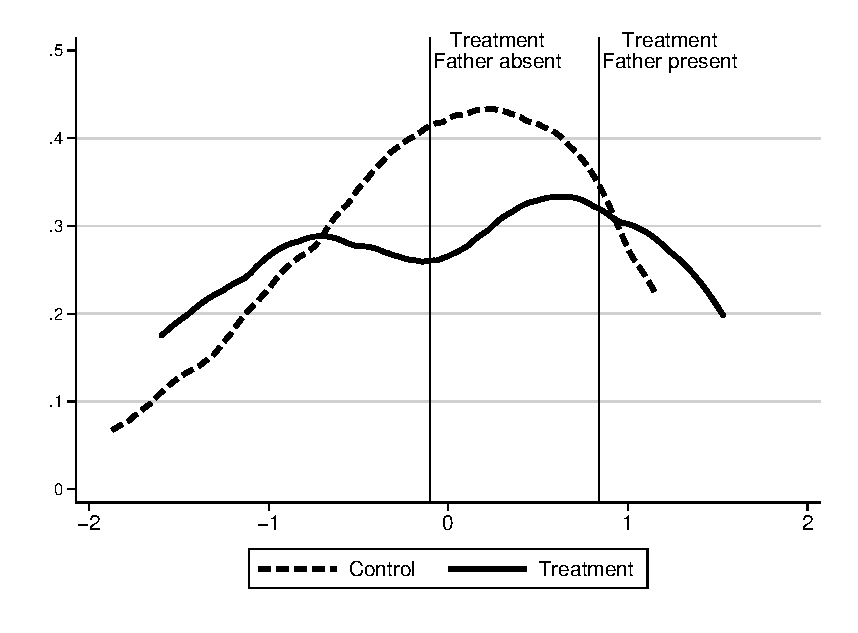
\includegraphics[width=\textwidth]{../output/HOME-males-factorhome}
	\end{subfigure}
	\begin{subfigure}[b]{0.49\textwidth}
		\centering
		\caption{Factor HOME Scores, Females}
		\label{fig:home-female-factor}
			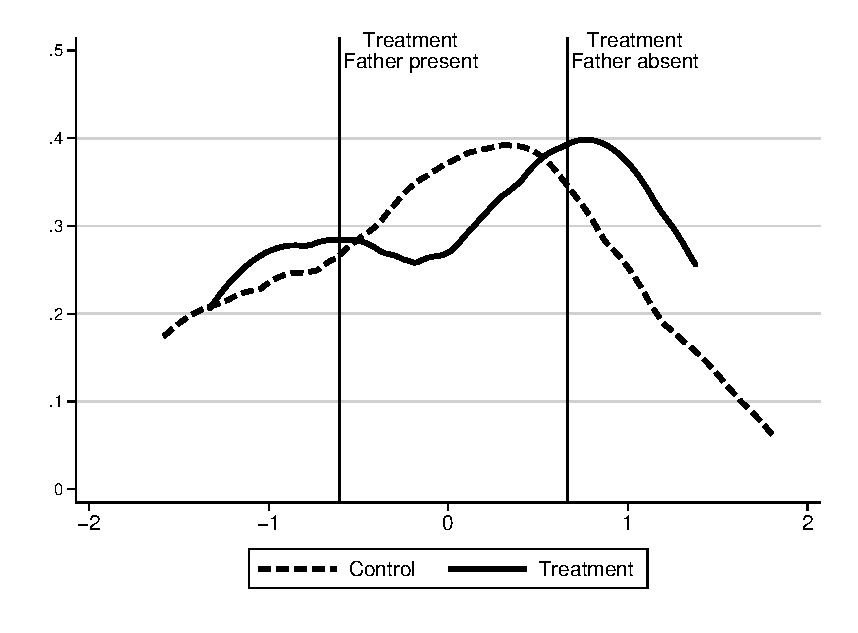
\includegraphics[width=\textwidth]{../output/HOME-females-factorhome}
	\end{subfigure}
\end{center}
\raggedright
Note: These plots show the distribution the factor of HOME scores. The factors are computed by gender using full HOME scores at 0.5, 1.5, 2.5, and 8 years. The vertical lines are the means of the treatment group by father's presence. 
\end{figure}

We explore this trend more closely in Figure~\ref{fig:total-home-quantiles}. To do so, we calculate the distribution pooling experimental groups but splitting by gender and father's presence. We then calculate, by gender and father's presence, the proportion of the treatment group that is in quantile 1 versus quantile 2. We do the same for the control group. 

The result of this exercise shows that the bimodal shape of the densities of the treatment group is explained differently by gender. For males, the HOME scores are higher for the control group when the fathers are absent and higher for the treatment group when father's are present. For females, the opposite is the case: The HOME scores are higher for the control group when fathers are present and higher for the treatment group when fathers are absent. 

One explanation of this is that treatment complements father's presence for males but substitutes it for females. Mothers then compensate for the father's absence for males (females) in the control (treatment) group. 

%One way mothers can compensate for the father's absence for males is to enroll them in alternate preschool arrangements. This is seen with more males in the control group being enrolled in these arrangements than control-group females (Figure~\ref{fig:alt-enrollment}). 

\begin{sidewaysfigure}
\begin{center}
\caption{Factor HOME Scores}
\label{fig:total-home-quantiles}
	\begin{subfigure}[b]{0.49\textwidth}
		\centering
		\caption{HOME, Father Absent, Males}
		\label{fig:home-male-mean}
			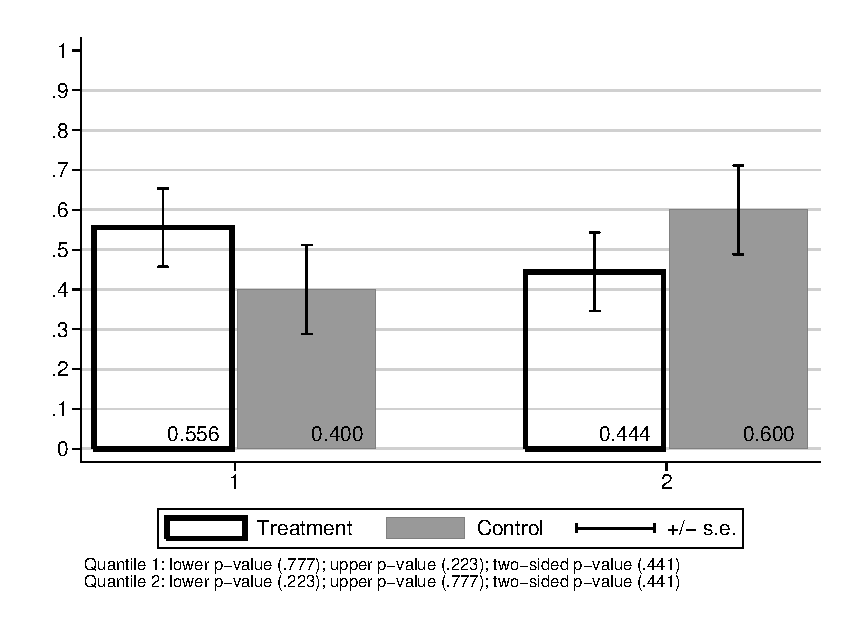
\includegraphics[width=\textwidth]{../output/HOME-male1-fhome0-2quant}
	\end{subfigure}
	\begin{subfigure}[b]{0.49\textwidth}
		\centering
		\caption{HOME, Father Absent, Females}
		\label{fig:home-female-mean}
			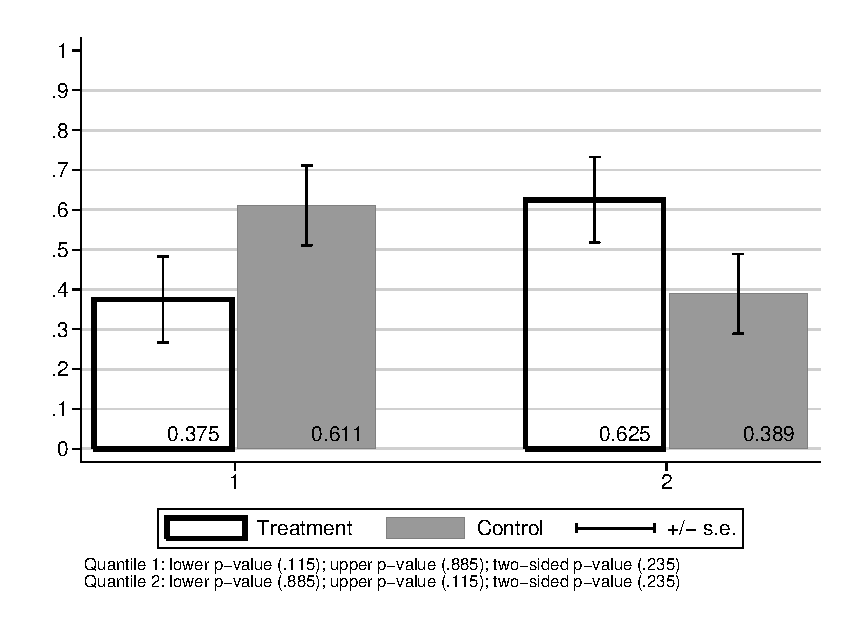
\includegraphics[width=\textwidth]{../output/HOME-male0-fhome0-2quant}
	\end{subfigure}
	
	\begin{subfigure}[b]{0.49\textwidth}
		\centering
		\caption{HOME, Father Present, Males}
		\label{fig:home-male-factor}
			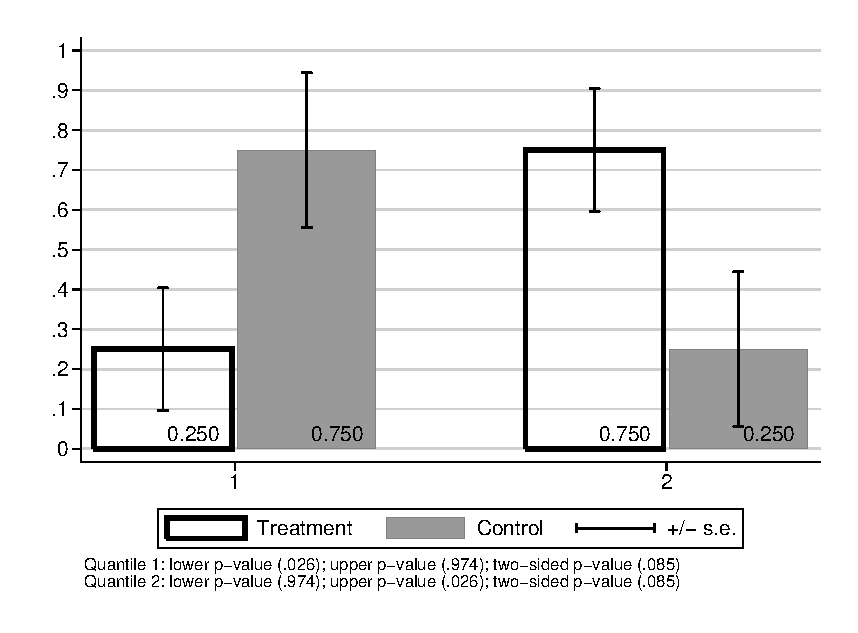
\includegraphics[width=\textwidth]{../output/HOME-male1-fhome1-2quant}
	\end{subfigure}
	\begin{subfigure}[b]{0.49\textwidth}
		\centering
		\caption{HOME, Father Present, Females}
		\label{fig:home-female-factor}
			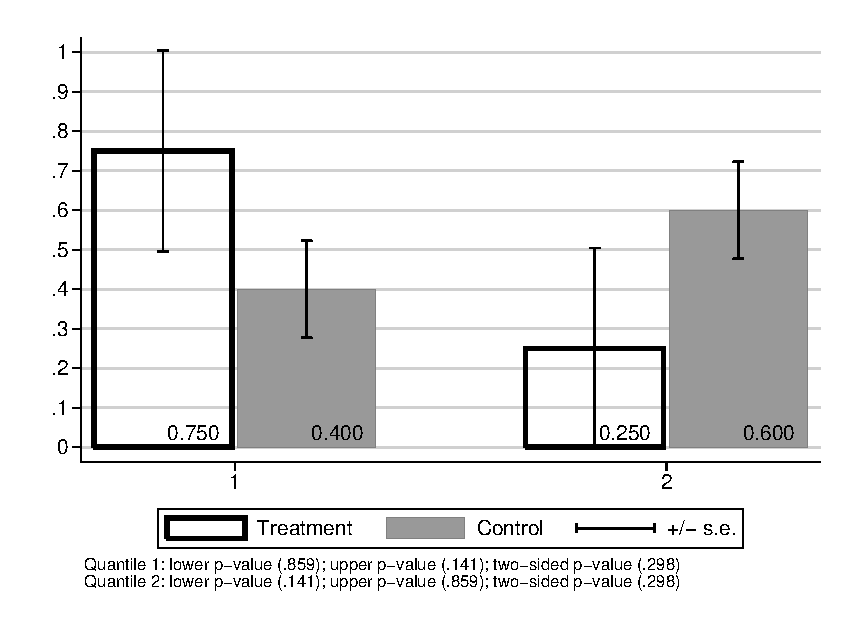
\includegraphics[width=\textwidth]{../output/HOME-male0-fhome1-2quant}
	\end{subfigure}
\end{center}
\raggedright \footnotesize
Note: The horizontal axis divides a factor of the HOME scores into the first and second quantile of the distribution pooling across experimental groups, but splitting  by gender and father's presence. The factors are computed by gender using full HOME scores at 0.5, 1.5, 2.5, and 8 years. The lower $p$-value tests that the treatment proportion is less than the control proportion within a quantile. The upper $p$-value tests that the treatment proportion is greater than the control proportion within a quantile. The numbers reported in the bars are the proportions. All standard errors and $p$-values are calculated using 1,000 bootstraps.
\end{sidewaysfigure}

%\begin{figure}
%\begin{center}
%\caption{Alternate Preschool Enrollment}
%\label{fig:alt-enrollment}
%	\begin{subfigure}[b]{0.49\textwidth}
%		\centering
%		\caption{Males by Father's Presence}
%			\includegraphics[width=\textwidth]{../output/family-dcmopre-father-male}
%	\end{subfigure}
%	\begin{subfigure}[b]{0.49\textwidth}
%		\centering
%		\caption{Females by Father's Presence}
%			\includegraphics[width=\textwidth]{../output/family-dcmopre-father-female}
%	\end{subfigure}
%	
%		\begin{subfigure}[b]{0.49\textwidth}
%		\centering
%		\caption{Pooled}
%			\includegraphics[width=\textwidth]{../output/family-dcmopre}
%	\end{subfigure}
%	\end{center}
%\raggedright
%Note: These histograms display the distributions of the months of enrollment in alternative preschool by gender. Months of enrollment are cumulative between birth and 5 years. 
%\end{figure}

